\section{Seguridad y control}

En este cap\'itulo veremos las caracter\'isticas de algunos elementos que son necesarios para realizar un control de la instalaci\'on y como operan cada uno de ellos. Tambi\'en se ver\'a como realizar operaciones de carga y vac\'io en la instalaci\'on.

\subsection{Man\'omentros}

En todo circuito frigor\'ifico hay que distinguir alta y baja presi\'on. Por lo tanto, tenemos man\'ometros para alta (color rojo) y para baja (color azul). Estos dispositivos a dem\'as de indicar presi\'on, indican la temperatura en funci\'on del fluido, como se puede ver en la siguiente figura.

\begin{figure}[H]
    \centering
    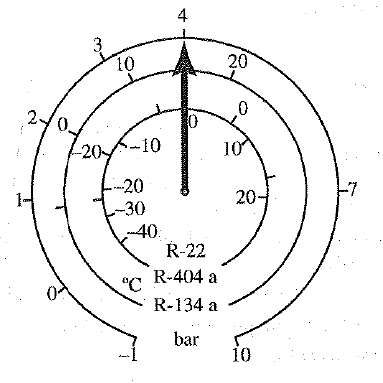
\includegraphics[width=.45\linewidth]{figuras/control-seguridad/manometro.png}
    \caption{Man\'ometro}
    \label{fig:manometro}
\end{figure}

\subsection{Analizador}  

\begin{wrapfigure}[4]{r}{0.4\linewidth}
    \centering
    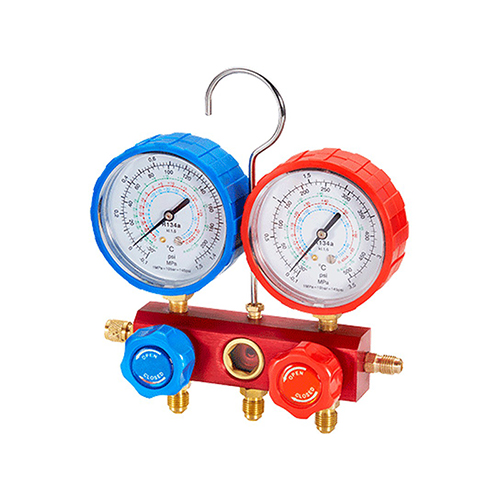
\includegraphics[width=.6\linewidth]{figuras/control-seguridad/analizador.jpg}
    \caption{Analizador}
    \label{fig:analizador}
\end{wrapfigure} 

Tambi\'en conocido como puente de man\'ometros. Nos sirve para ``comunicarnos'' con el circuito, ya que al conectarlo se pueden analizar operaciones tales como: 

\begin{itemize}
    \item Comprobar presiones de trabajo
    \item Meter y sacar fluido refrigerante
    \item Hacer vac\'io a un determinado tramo de la instalaci\'on o a su totalidad
\end{itemize}

Consta de un cuerpo (analizador) que, por lo general, tiene:

\begin{itemize}
    \item Dos v\'alvulas, una de color azul y otra de color rojo.
    \item Dos man\'ometros, alta y baja presi\'on.
    \item Un juego de mangueras, azul (baja), roja (alta) y amarilla (carga, descarga o vac\'io).
    \item Una mirilla en la parte central.
\end{itemize}

\begin{figure}[H]
    \centering
    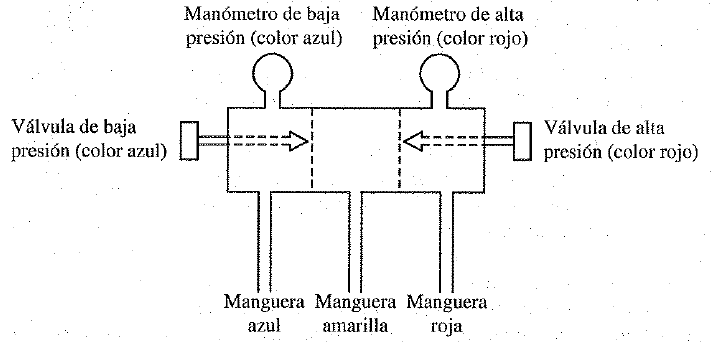
\includegraphics[width=.6\linewidth]{figuras/control-seguridad/analizador-partes.png}
    \caption{Esquema del analizador}
    \label{fig:esquema-analizador}
\end{figure}

En el esquema se puede observar que al estar las dos v\'alvulas abiertas est\'an comunicadas la baja presi\'on, la alta y la manguera amarilla (que estar\'a conectada a la bomba de vac\'io o a la botella de refrigerante).

\textbf{Manguera azul}

La conectamos a un punto del ciruito de baja presi\'on, por ejemplo a la v\'alvula de servicio de aspiraci\'on del compresor, y con la v\'alvula del analizador cerrada, el man\'ometro nos marca la presi\'on de aspiraci\'on del compresor, puesto que al cerrar la v\'alvula, impide que el fluido pase hacia las mangueras amarilla y roja.

\textbf{Manguera roja}

La conectamos a un punto del circuito de alta presi\'on, por ejemplo a la v\'alvula de servicio de descarga (tambien a su toma exterior), y con la v\'alvula del analizador cerrada, el man\'ometro nos indica la presi\'on de descarga, asi como la temperatura de condensaci\'on.

\textbf{Manguera amarilla}

Es para realizar operaciones que se consideren oportunas, como por ejemplo, conectarla a la bomba de vac\'io o a la botella de refrigerante por si queremos meter o sacar carga.

\subsection{Detector de fugas}

Las fugas pueden ser debidas a un error en el montaje, por ejemplo una soldadura mal realizada, o producirse durante el funcionamiento de la instalaci\'on. En este \'ultimo caso, principalmente son por falta de mantenimiento adecuado, ya que, por ejemplo, la existencia de aire o de humedad favorecen a los problemas de corrosi\'on y, por lo tanto, el deterioro de ciertos elementos que sometidos a las presiones de trabajo provocan poros en tuber\'ias que dan lugar a fugar del fluido refrigerante. \textbf{Las fugas implican disminuciones de las presiones de trabajo, y en el visor ver\'iamos pasar burbujas. Uno de los s\'intomas que indican que hay fugas en un punto del circuito es cuando se encuentra aceite en el exterior del elemento o tramo de tuber\'ia.}

Para la localizaci\'on de las fugas se puede recurrir a varios tipos de detectores, entre los que cabe citar:

\begin{enumerate}[a)]
    \item \textbf{L\'ampara hal\'ogena}\\ Consta de una botella de butano que calienta un filamento de cobre, y en un extremo tiene un tubo de goma que lo orientamos hacia los punto que queremos comprobar. En caso de encontrar una fuga de fluido refrigerante, la llama de la botella que es de color azul cambia a verde. La intensidad del color es funci\'on de la cantidad de fluido que detecte.
    \item \textbf{Detector electr\'onico}\\ Estos detectores tienen una gran precisi\'on. Por su gran sensibilidad, son muy adecuados para la detecci\'on de fugas muy pequeñas. Emiten señales ac\'usticas y visuales.
    \item \textbf{Agua jabonosa}\\ Consiste en formar agua jabonosa en un pequeño recipiente y a mano o con ayuda de un pequeño pincel, se cubre el elemento o tramo de la instalaci\'on a comprobar. En caso de detectarse alguna fuga se formar\'an burbujas.
    \item \textbf{Listoncitos de madera impregnados de azufre}\\ En instalaciones de amon\'iaco se suelen emplear listoncitos de madera impregnados de azufre, que al ponerse en contacto con el amon\'iaco entra en combusti\'on y arden. Las fugas de este fluido se detectan f\'acilmente por su fuerte olor acre.
    \item \textbf{Introducci\'on de c\'apsulas flourescentes en el cirucuito}\\ Consiste en la introducci\'on en el circuito de un aditivo flourescente de acuerdo con el fluido refrigerante de la instalaci\'on. A continucaci\'on se realiza un cequeo de la instalaci\'on con una l\'ampara U.V., es un sistema de gran precisi\'on.
\end{enumerate}

\subsection{V\'alvulas de servicio}

Se emplean en compresores herm\'eticos, semiherm\'eticos y abiertos. Pueden ser de aspiraci\'on o de descarga. Son v\'alvulas de tres v\'ias que comunican el interior del circuito con el exterior para poder realizar operaciones tales como comprobar presiones o meter carga de refrigerante. Existen las v\'alvulas de servicio de aspiraci\'on (inferior) y de descarga (superior) como se puede observar en la \autoref{fig:valvulas-servicio-compresor}.

\begin{figure}[H]
    \centering
    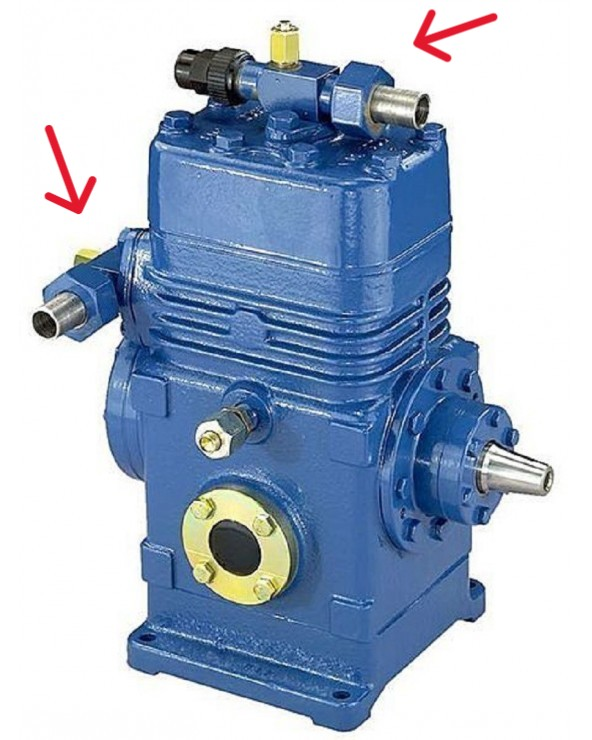
\includegraphics[width=.6\linewidth]{figuras/control-seguridad/valvulas-servicio.jpg}
    \caption{V\'alvulas de servicio en un compresor abierto}
    \label{fig:valvulas-servicio-compresor}
\end{figure}

\subsubsection{V\'alvulas de servicio de aspiraci\'on}

Tal como se aprecia en la \autoref{fig:valvula-servicio-aspiracion}, est\'an montadas en el mismo compresor. Se tiene que:

\begin{itemize}
    \item La conexi\'on (A), que es la aspiraci\'on del compresor
    \item Una segunda conexi\'on (B), que une la v\'alvula con la tuber\'ia de baja presi\'on procedente del evaporador
    \item Y la tercera conexi\'on (C), de tap\'on roscado, es para la comunicaci\'on con el exterior, a la que podemos acoplar, por ejemplo, un analizador para meter carga en estado de gas o un man\'ometro para comprobar la presi\'on de aspiraci\'on del compresor
\end{itemize}

\begin{figure}[H]
    \centering
    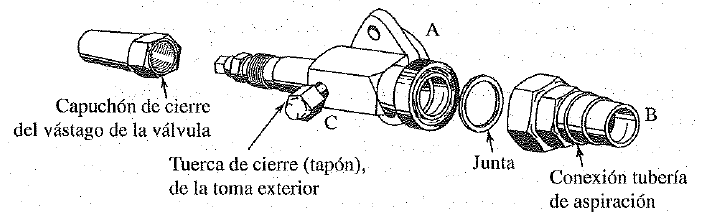
\includegraphics[width=.6\linewidth]{figuras/control-seguridad/valvula-servicio-aspiracion.png}
    \caption{V\'alvula de servicio de aspiraci\'on}
    \label{fig:valvula-servicio-aspiracion}
\end{figure}

\textbf{Funcionamiento:}

\begin{enumerate}[1.]
    \item Al abrir totalmente la v\'alvula, el compresor y la tuber\'ia de baja presi\'on (evaporador) est\'an comunicados; pero la toma exterior est\'a incomunicada (cerrada).
    \item Al cerrar totalmente la v\'alvula, el compresor y la tuber\'ia de baja presi\'on quedan incomunicados; pero la toma exterior est\'a comunicada con el compresor.
    \item Siempre que la v\'alvula no est\'e ni cerrada ni abierta en su totalidad, estar\'an las tres conexiones comunicadas, es decir, el compresor, el evaporador y la toma exterior.
\end{enumerate}

En caso de querer colocar un man\'ometro para saber la presi\'on y temperatura de aspiraci\'on el proceso es el siguiente:

\begin{enumerate}[1.]
    \item Se saca el capuch\'on de cierre del v\'astago de la v\'alvula y comprueba que est\'e abierta en su totalidad. Para ello, se gira el v\'astago de la v\'alvula a fundo (en sentido contrario a las agujas del reloj)
    \item Se saca el tap\'on de la toma exterior de la v\'alvula, pues \'esta est\'a cerrada (incomunicada), y se conecta el man\'ometro
    \item Se cierra la v\'alvula un poco (en sentido de las agujas del reloj) y el man\'ometro ya marcar\'a la presi\'on de aspiraci\'on
\end{enumerate}

Asimismo, la v\'alvula de servicio de aspiraci\'on se emplea para realizar la carga de la instalaci\'on con fluido refrigerante en estado de gas. 

\textbf{Operaci\'on de carga de fluido refrigerante en estado de gas}

La carga se puede realizar conectando directamente la botella del refrigerante a la v\'alvula de servicio o atrav\'es de un analizador \autoref{fig:carga-fluido-gas}:

\begin{enumerate}[1.]
    \item Se conecta la manguera azul a la toma exterior de la v\'alvula de servicio de aspiraci\'on sin apretar la conexi\'on a fondo
    \item Se comprueba que la v\'alvula roja del analizador est\'e cerrada. Se abre la v\'alvula azul del analizador
    \item Se abre despacio la v\'alvula de la botella de refrigerante
    \item Se realiza el ``purgado'' de toda la l\'inea (que consiste en eliminar el aire que contienen las mangueras, desde la botella hasta la conexi\'on en la v\'alvula de servicio). Cuando salga refrigerante, se aprieta a fondo la conexi\'on en la toma exterior de la v\'alvula de servicio
    \begin{figure}[H]
        \centering
        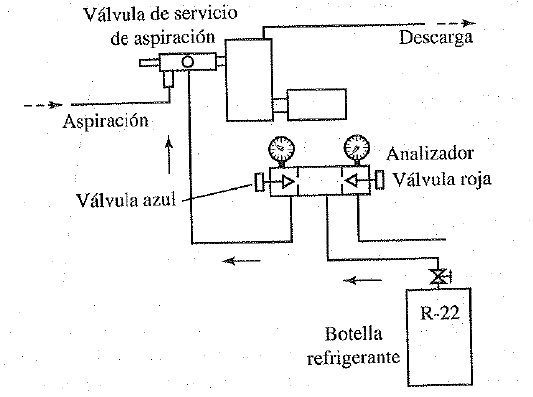
\includegraphics[width=.5\linewidth]{figuras/control-seguridad/carga-fluido-gas.png}
        \caption{Carga de fluido refrigerante a trav\'es del analizador}
        \label{fig:carga-fluido-gas}
    \end{figure}
    \item Se abre despacio la v\'alvula de servicio de aspiraci\'on. Se comienza a cargar el circuito de fluido
    \item Al cerrar la v\'alvula azul del analizador, se interrumpe la entrada del fluido refrigerante. La presi\'on que marca el man\'ometro, es la presi\'on de aspiraci\'on del compresor, lo que nos da una referencia de la carga introducida
    \item Al finalizar la carga, y para que el compresor aspire todo el fluido de las mangueras, se cierra la v\'alvula de la botella de refrigerante y se abre totalmente la v\'alvula de servicio de aspiraci\'on
\end{enumerate}

\subsubsection{V\'alvula de descarga}

Constructivamente es identica a la v\'alvula de aspiraci\'on pero la diferencia es que comunica otras partes del circuito.

\textbf{Funcionamiento:}

\begin{enumerate}[1.]
    \item Cuando la v\'alvula est\'a totalmente abierta, el compresor y condensador est\'an comunicados entre s\'i, pero la toma exterior est\'a incomunicada
    \item Cuando la v\'alvula est\'a totalmente cerrada, el compresor y el condensador est\'an incomunicados, pero el compresor est\'a comunicado con la toma exterior (para que se pueda conectar un man\'ometro, analizador, etc.)
    \item Siempre que la v\'alvula no est\'e a fondo, en sus posiciones de aberura o cierre, las tres conexiones estar\'an comunicadas
\end{enumerate}

Esta v\'alvula se utiliza para medir/verificar la presi\'on de descarga del compresor.

\subsubsection{V\'alvula rotalock}

Es una v\'alvula como las de servicio de aspiraci\'on y descarga pero se la coloca entre el recipiente de l\'iquido y el evaporador. Al estar abierta la v\'alvula comunica estos dos dispositivos. Con la ayuda de esta v\'alvula y una de carga se puede realizar la carga de refrigerante en estado l\'iquido.

\begin{figure}[htbp]
    \centering
    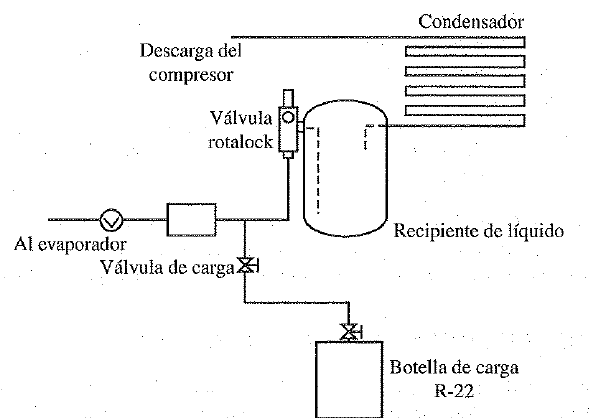
\includegraphics[width=.6\linewidth]{figuras/control-seguridad/carga-fluido-liquido.png}
    \caption{Carga de refrigerante en estado l\'iquido}
    \label{fig:carga-fluido-liquido}
\end{figure}

\textbf{Operaci\'on de carga de refrigerante en estado l\'iquido}

La \autoref{fig:carga-fluido-liquido} muestra la configuraci\'on de las v\'alvulas para que se puede realizar la operaci\'on. Este procedimiento se puede realizar sin parar el funcionamiento de la instalci\'on. Se puede realizar de la siguiente manera:

\begin{enumerate}[1.]
    \item Se conecta un man\'ometro a la toma exterior de la v\'alvula rotalock. Siguiendo los pasos necesarios.
    \item Se conecta la botella de refrigerante, mediante la manguera, a la v\'alvula de carga. La conexi\'on de la manguera se realiza sin apretar a fondo (parcialmente roscada)
    \item Se abre despacio la v\'alvula de la botella y cuando salga fluido refrigerante por la conexi\'on de la manguera, se aprieta a fondo (se enrosca totalmente). De esta manera se purga la manguera
    \item Se cierra la v\'alvula rotalock, el compresor al estar en funcionamiento recoge el fluido en el circuito que existente entre la v\'alvula rotalock y el evaporador.
    \item Una vez que se visualiza en el man\'ometro que la presi\'on del circuito esta por debajo de la presi\'on de la botella de refrigerante, se procede abrir la v\'alvula de carga. Se comienza a cargar la instalaci\'on.
    \item Cuando el nivel de l\'iquido en el recipiente de l\'iquido llegue a su valor deseado se procede a cerrar la v\'alvula de la botella.
    \item Se cierra la v\'alvula de carga y se abre totalmente la v\'alvula rotalock
\end{enumerate}

\subsection{V\'alvula solenoide}

Son electrov\'alvulas normalmente cerradas o normalmente abiertas. Su funci\'on principal es permitir o restringir el flujo del refrigerante ante ciertas situaciones del sistema, su regulaci\'on es todo-nada. Generalmente son normalmente cerradas y utilizan la presi\'on del sistema para mantenerse cerradas. En cuanto a su conexi\'on pueden ser rosacadas o soldadas.

Sus partes se pueden observar en la siguiente figura:
\begin{figure}[H]
    \centering
    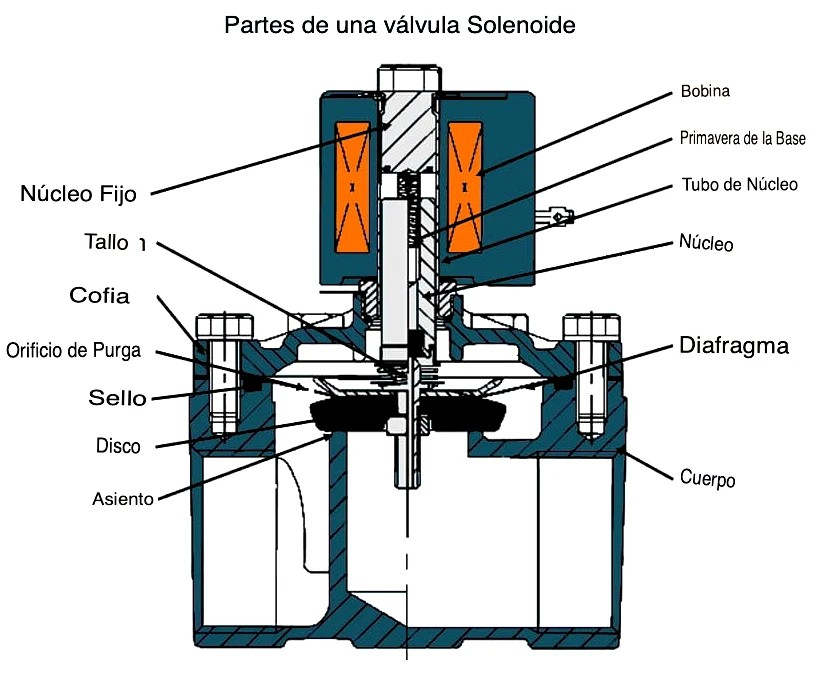
\includegraphics[width=0.6\linewidth]{figuras/control-seguridad/valvula-soleinoide.jpg}
    \caption{Partes de una v\'alvula solenoide}
    \label{fig:partes-valvula-solenoide}
\end{figure}

La apertura de la v\'alvula se realiza alimentado la bobina solenoide, la cual crea un campo magn\'etico que mueve el bastago (electroim\'an) para permitir el paso del fluido.

Esta v\'alvula se la utiliza para realizar diferentes acciones sobre el sistema:

\begin{itemize}
    \item \textbf{Parada de compresor:}\ Cuando se est\'a por apagar el compresor, se cierra la v\'alvula solenoide y el compresor comienza a vaciar el evaporador del fluido refrigerante. Esto causa una disminuci\'on de presi\'on en la l\'inea de succi\'on y cuando se llega al valor m\'inimo seteado, el presostato de baja apaga el compresor. Este sistema de apagado se conoce como \textit{Pump Down}.
    \item \textbf{Desescarche de gas:}\ Permite el flujo de refrigerante en estado gaseoso a alta presi\'on hacia el evaporador, antes de la v\'alvula termost\'atica de expasi\'on.
    \item \textbf{Varios evaporadores:}\ Se utilizan cuando tenemos varios evaporadores que refrigeran diferentes ambientes, se utiliza una para alimentar cada evaporador.
\end{itemize}

\subsection{Presostato diferencial de aceite}

Es un tipo de presostato muy especial, cuya funci\'on es la de medir la diferencia de presi\'on entre la presi\'on de aceite de la bomba del compresor y la presi\'on del c\'arter o de succi\'on del sistema, de forma que si hay fallas de lubricaci\'on, este cambia sus contactos internos, de forma que se puede apagar el compresor.

A diferencia de los presostatos de presi\'on, estos poseen un bimet\'alico interno que act\'ua de temporizador para que al momento de sentirse la baja presi\'on, se activa el tiempo de conteo y al final los contactos cambian o conmutan. Es muy importante este tipo de tamporizaci\'on, sobre todo en los arranques, porque la presi\'on de succi\'on es inestable y requiere un tiempo para estabilizarse. 

\begin{figure}[H]
    \centering
    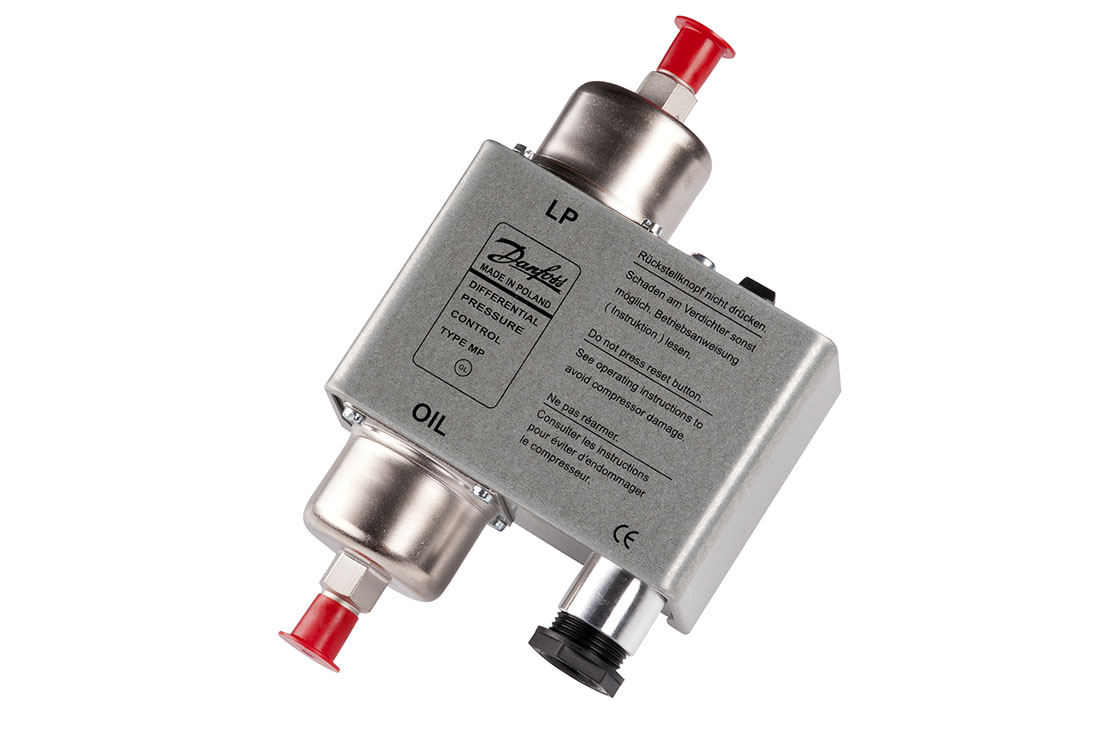
\includegraphics[width=.6\linewidth]{figuras/control-seguridad/presostato-diferencial-aceite.jpg}
    \caption{Presostato diferencial de aceite}
\end{figure}

\textbf{Funcionamiento.}\ En caso de que disminuya la presi\'on de descarga de la bomba de aceite, por falta de aceite o porque el filtro se encuentra sucio, haciendo caer el diferencial de presi\'on por debajo del seteado, el presostato apagar\'a el compresor.

\subsection{Protector t\'ermico}

Este accesorio es un contacto normalmente cerrado, que va conectado en serie con el punto com\'un del compresor. En el circuito el\'ectrico de un motor monof\'asico, la fase se conecta al protector y luego al contacto com\'un.

\begin{wrapfigure}[8]{r}{0.4\linewidth}
    \centering
    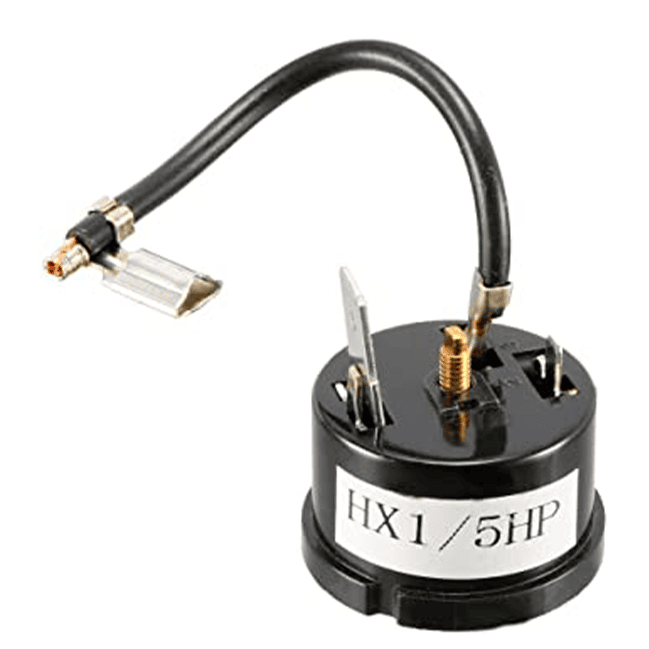
\includegraphics[width=0.4\linewidth]{figuras/control-seguridad/protector-termico.png}
    \caption{Protector t\'ermico}
    \label{fig:protector-termico}
\end{wrapfigure}

Este dispositivo en los compresores de baja potencia es externo al compresor, pero en los compresores de media a alta potencia, va ubicado en el interior de los mismos. 

En situaciones de temperatura del c\'arter o carcaza normal, con corrientes normales, el protector t\'ermico esta cerrado permitiendo la operaci\'on del compresor. En caso de que estas aumenten a un valor tal que sea peligroso para la bobina de la m\'aquina, este dispositivo abrir\'a el circuito el\'ectrico. Esto sucede porque contiene un disco bimet\'alico que se arquea cuando esta expuesto a altas temperaturas, abriendo as\'i el circuito.

En la siguiente figura se pueden observar los componentes internos del protector:

\begin{figure}[H]
    \centering
    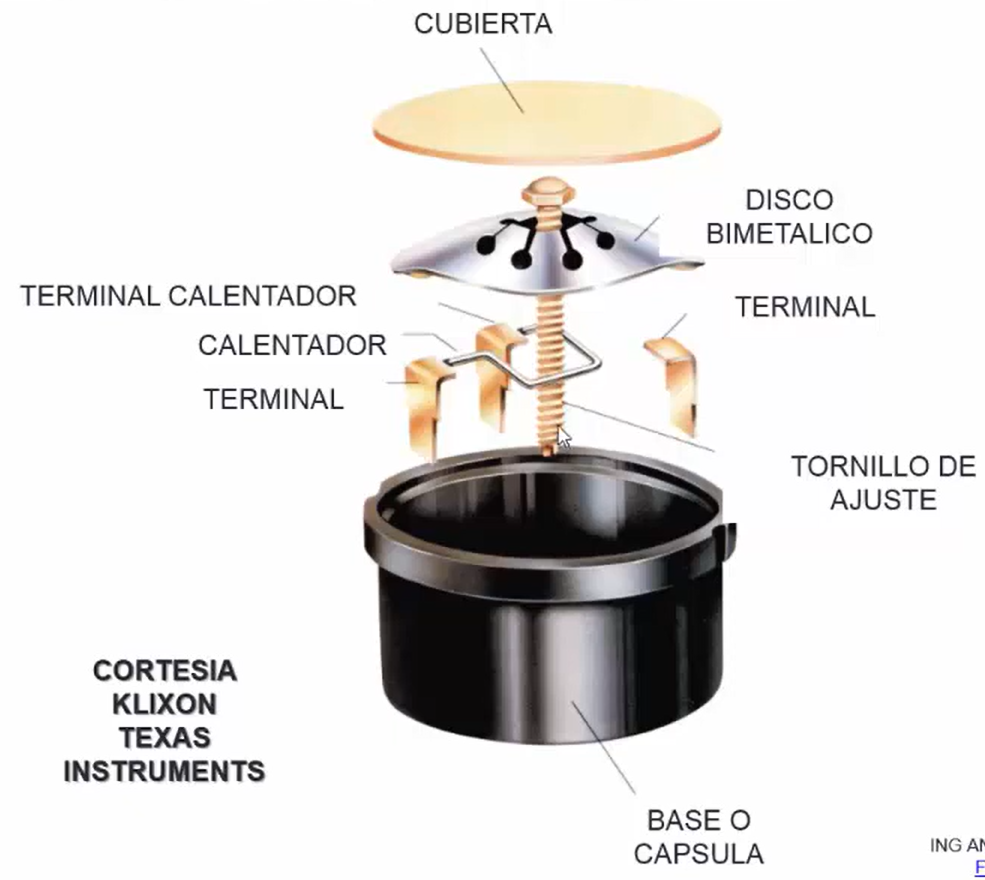
\includegraphics[width=.4\linewidth]{figuras/control-seguridad/partes-protector-termico.png}
    \caption{Partes protectos t\'ermico}
\end{figure}
